\FloatBarrier
\section{Metodología Aplicada}%
\label{sec:methodology}

\begin{corregir}

Para estructurar las fases de desarrollo del proyecto y la gestión de los objetivos específicos se aplicará una
combinación de \textit{Scrum} con \textit{Crisp-DM}.
Se detallan a continuación ambas metodologías, junto con las técnicas y herramientas a utilizar:

\textit{Scrum} es un marco de trabajo que posibilita un proceso ágil y liviano para administrar y controlar el
desarrollo de \textit{software}.
Es iterativo e incremental y cada iteración o \textit{sprint} concluye con una pieza de \textit{software} ejecutable que
incorpora nueva funcionalidad.

Se deben aplicar ciertas modificaciones ya que el equipo de trabajo estará conformado por un único integrante (también
conocido como \textit{Single Scrum}), destacando que el autor del proyecto combinará los roles de Desarrollador,
\textit{Product Owner} y \textit{Scrum Master}.

En principio se planean seis \textit{sprints} con una duración de dos semanas cada una, de forma que la totalidad del
proyecto contempla una duración aproximada de tres meses.
Una vez definidas las historias de usuario se deberá proceder a dividirlas en tareas más pequeñas que terminarán
formando parte del \textit{backlog} del proyecto.

Al finalizar cada \textit{sprint} se compartirá el avance hasta el momento con el/la tutor/a del proyecto para obtener
la retroalimentación correspondiente.

Si bien su aplicación abarca la totalidad de las tareas del proyecto, se destaca para las potenciales tareas del
desarrollo de \textit{software} que serán necesarias en este proyecto como la implementación del \textit{endpoint} que,
a partir del contenido de un correo electrónico, extraiga la información relevante y también la implementación de una
interfaz web simple que muestre el itinerario agregado de un usuario.

\textit{Crisp-DM} es una metodología para el desarrollo de proyectos de \textit{data mining} (DM) independiente de las
herramientas de \textit{software}.
Esta metodología estructura el trabajo en seis fases: Comprensión del negocio, Análisis de los datos, Preparación de los
Datos, Modelado, Evaluación y Despliegue.
Su aplicación permitirá en este proyecto guiar la potencial creación de modelos de clasificación de los correos
electrónicos, la implementación de técnicas de extracción de información y la evaluación de los resultados obtenidos.

\end{corregir}

\subsection{Técnicas y Herramientas}%
\label{subsec:tools}

\begin{corregir}

En cuanto a las técnicas, en primer lugar se utilizarán tokenización y normalización, provenientes del área del
procesamiento de lenguaje natural (NLP). Para la clasificación de los correos electrónicos según el tipo de reserva que
contengan se utilizarán modelos de aprendizaje supervisado.
También se utilizará Named Entity Recognition para poder extraer la información relevante de cada mail de reserva, con
la ayuda de expresiones regulares para aquellos casos que respeten patrones predecibles.

Respecto al desarrollo de la solución se utilizarán diversas herramientas de acuerdo con los requerimientos de cada
componente.
Para el proceso de extracción, transformación y carga (ETL) se utilizará principalmente el lenguaje de programación
Java.
También se utilizará el lenguaje de programación R para los modelos de clasificación y extracción.
La visualización de los resultados se llevará a cabo utilizando Observable.
Para la implementación de la aplicación web que muestra el itinerario consolidado del usuario se utilizará Spring Boot.
Se evaluará además la posibilidad de incorporar un orquestador de flujos de trabajo como Apache Airflow.

Por otro lado, para la organización del proyecto en general se utilizarán varias funcionalidades del sitio GitHub.com
destacando el versionado del código fuente con \textit{Git} y el manejo del \textit{backlog} con GitHub Projects.
Se detallan a continuación ambas herramientas:

\end{corregir}

\subsubsection{Git}

\begin{revisado}

Git es una herramienta de control de versión ampliamente utilizada en la industria del \textit{software} que permite
llevar un registro de todos los cambios realizados en el tiempo.

Se creará un repositorio privado en~\cite{github} que actuará como servidor remoto del repositorio Git local.

En este proyecto su aplicación permitirá revertir cambios cuando sea necesario, trabajar en distintas funcionalidades de
manera paralela mediante el uso de ramas o \textit{branches} y organizar la creación de los entregables de cada
\textit{sprint} mediante la funcionalidad de \textit{releases} y \textit{tags}.

\end{revisado}

\subsubsection{GitHub Projects}

\begin{revisado}

Las incidencias o \textit{issues} serán la herramienta para crear cada una de las tareas que formarán parte del
\textit{backlog}.
Cada \textit{issue} (Ver \autoref{fig:github-issues}) cuenta con una descripción y referencias a los cambios realizados
en el código fuente para resolver esa tarea, además de poder categorizarlas con etiquetas o \textit{labels}.

\end{revisado}

\begin{figure}[htbp]
    \centering
    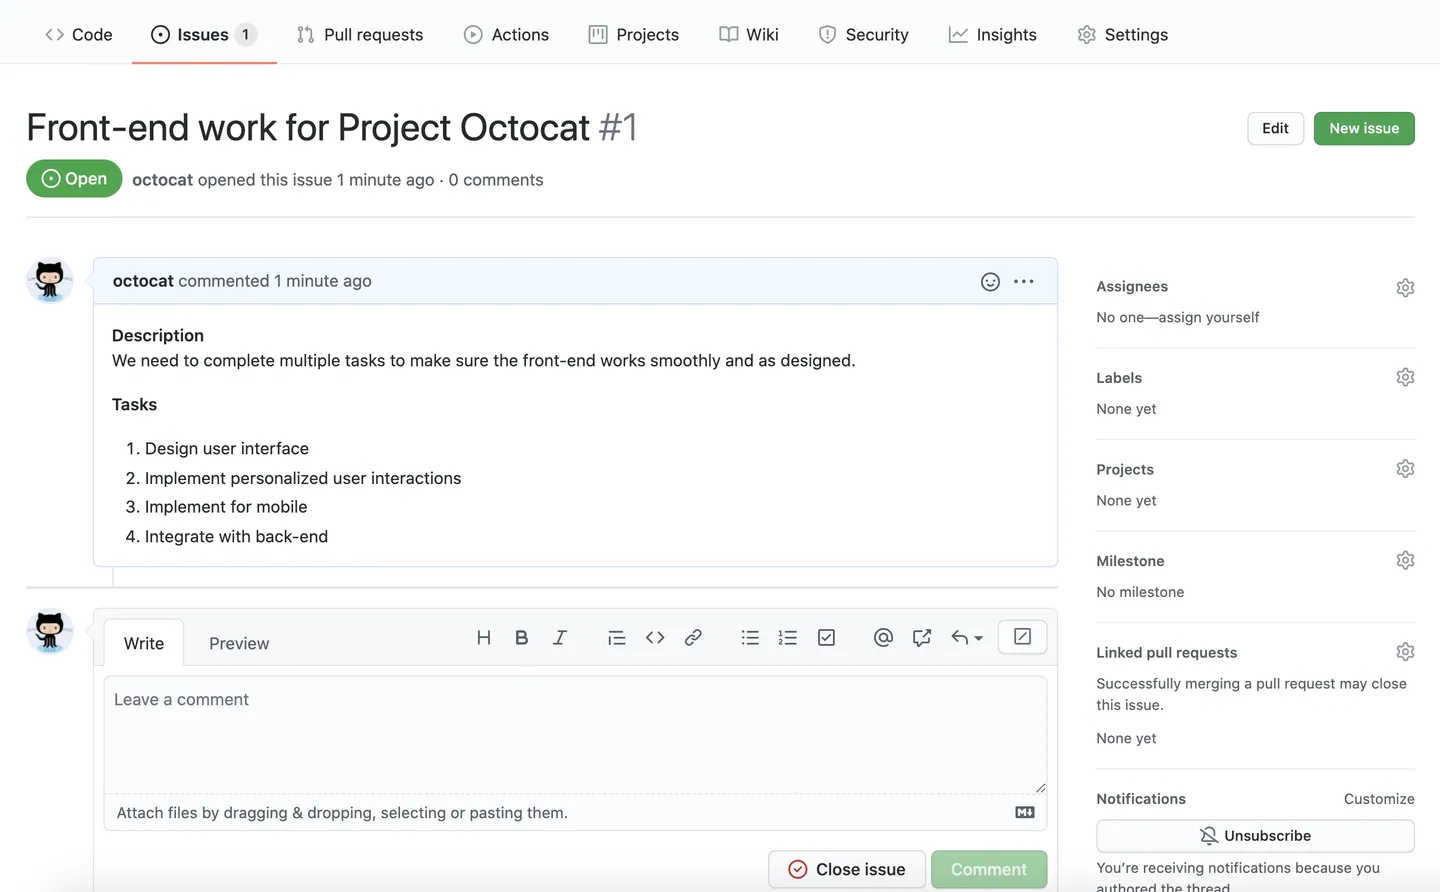
\includegraphics[width=1.00\textwidth]{images/github-issues}
    \caption{Captura de ejemplo de una \textit{issue} del proyecto extraída de la documentación oficial de GitHub}%
    \label{fig:github-issues}
\end{figure}

\begin{revisado}

GitHub Projects permite organizar el desarrollo mediante tableros Kanban que estarán poblados por cada una de las
\textit{issues} del proyecto.
En una vista general del tablero o \textit{board layout} (Ver \autoref{fig:github-projects-board}) se pueden distinguir
las \textit{issues} por estado: si están todavía pendientes de análisis, en desarrollo, en etapa de pruebas o ya
finalizada dado que ya fueron integradas a la implementación final.

\end{revisado}

\begin{figure}[htbp]
    \centering
    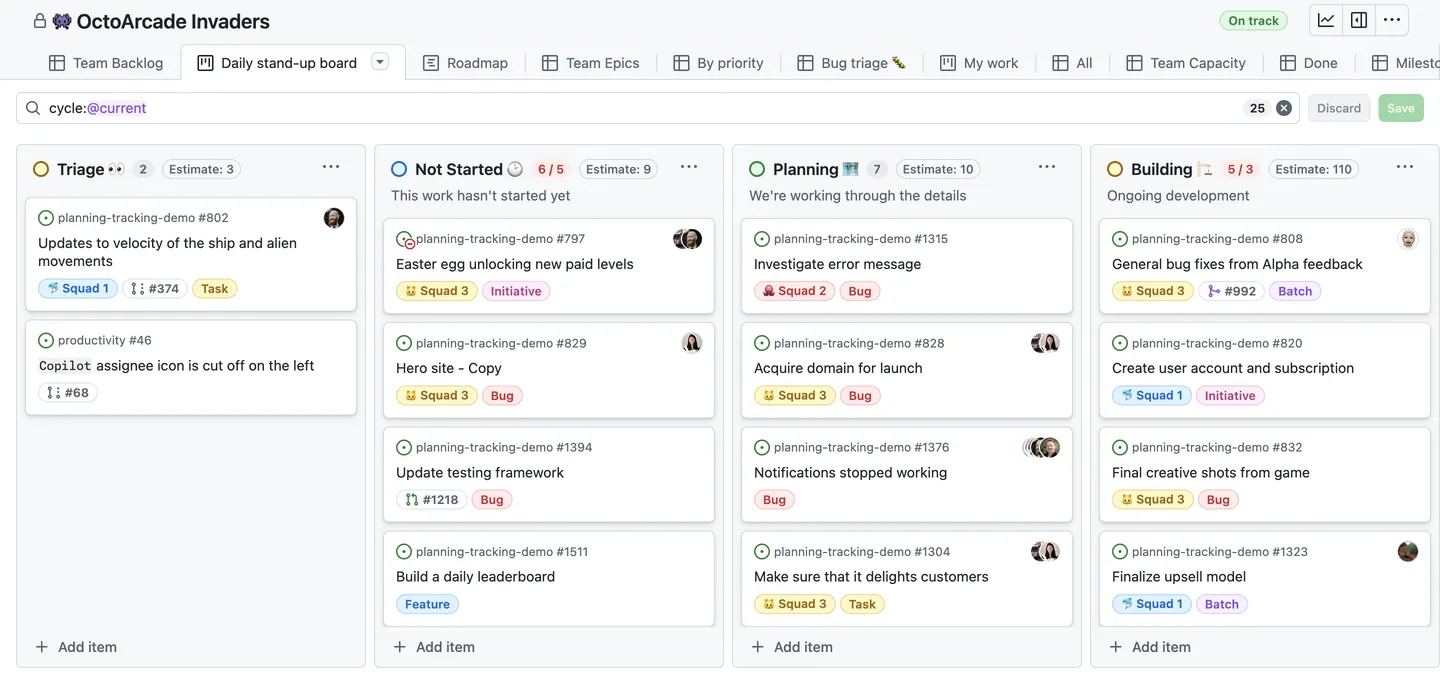
\includegraphics[width=1.00\textwidth]{images/github-projects-board}
    \caption{Captura de ejemplo de una vista \textit{board} del proyecto extraída de la documentación oficial de GitHub}%
    \label{fig:github-projects-board}
\end{figure}

\begin{revisado}

También se ofrece una vista del ciclo de vida de desarrollo o \textit{roadmap}
(Ver \autoref{fig:github-projects-roadmap}) donde se puede apreciar la dimensión tiempo en cantidad de semanas y cómo
las tareas se fueron resolviendo en cada momento.

\end{revisado}

\begin{figure}[htbp]
    \centering
    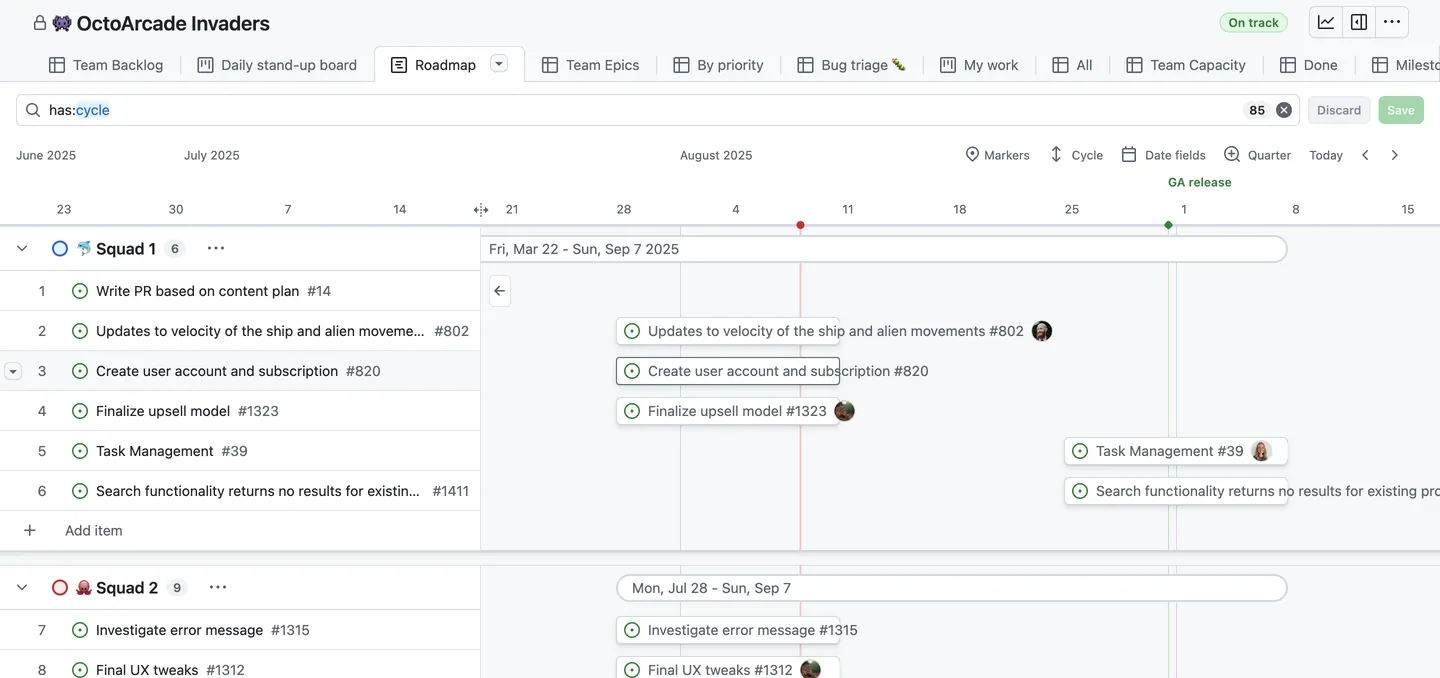
\includegraphics[width=1.00\textwidth]{images/github-projects-roadmap}
    \caption{Captura de ejemplo de una vista \textit{roadmap} del proyecto extraída de la documentación oficial de
    GitHub}%
    \label{fig:github-projects-roadmap}
\end{figure}

\subsection{Preparación de los Datos}%
\label{subsec:data-preparation}

\subsection{Análisis Exploratorio de los Datos}%
\label{subsec:eda}
